\documentclass[
  11pt,
  letterpaper,
   addpoints,
   answers
  ]{exam}

\usepackage{../exercise-preamble}
\usepackage{float}
\begin{document}

\noindent
\begin{minipage}{0.47\textwidth}

\includegraphics[width=\textwidth]{../fcfm_die}
\end{minipage}
\begin{minipage}{0.53\textwidth}
\begin{center} 
\large\textbf{Conversión de la Energía y Sistemas Eléctricos } (EL4111-1) \\
\large\textbf{Clase auxiliar Examen} \\
\small Prof.~Constanza Ahumada - Rodrigo Moreno.\\
\small Prof.~Aux.~Javiera Pacheco - Erik Sáez\\
\small Ayudantes.~Manuel Aceituno - Pamela Acuña - Alvaro Flores\\
\end{center}
\end{minipage}

\vspace{0.5cm}
\noindent
\vspace{.85cm}

\begin{questions}
    \question \textbf{Preguntas conceptuales}.\\\\
    Preguntas de motor de inducción
    \begin{enumerate}
        \item ¿Cuál es la diferencia entre el comportamiento de un motor de inducción trifásico en condiciones de vacío y en condiciones de rotor bloqueado? Explica cómo estas pruebas ayudan a determinar los parámetros del circuito equivalente.
    
        \item ¿Por qué el deslizamiento (\(s\)) en un motor de inducción es diferente entre el arranque y el régimen permanente? Explica cómo este parámetro influye en el torque del motor.
    
        \item En un motor de inducción, ¿cómo afecta la conexión en estrella o en delta la tensión y la corriente de línea? Explica las ventajas de cada tipo de conexión.
    
        \item ¿Qué parámetros del circuito equivalente del motor de inducción pueden determinarse a partir de las pruebas de vacío y rotor bloqueado? Describe el procedimiento para obtenerlos.
    
        \item ¿Cómo se calcula el torque máximo en un motor de inducción y qué relación tiene este valor con el deslizamiento? Explica la importancia de este punto en el diseño y operación del motor.
    
        \item ¿Cuál es la principal diferencia en el principio de funcionamiento entre un motor síncrono y un motor de inducción? Explica cómo estas diferencias afectan su aplicación en sistemas eléctricos.
    \end{enumerate}
    Preguntas de SEP
    \begin{enumerate}
        \item ¿Qué ventajas tiene el uso de valores en por unidad en los sistemas eléctricos de potencia?
    
        \item ¿Cómo se define la base común en un SEP trifásico y cómo se calculan las magnitudes base?
    
        \item ¿Qué simplificaciones se realizan al modelar un sistema eléctrico en régimen permanente?
    
        \item ¿Qué elementos deben considerarse al resolver un SEP trifásico mediante su equivalente monofásico?
    
        \item ¿Cuáles son las formas típicas de modelar las líneas de transmisión?
    \end{enumerate}

    Preguntas de ERNC

    \begin{enumerate}
        \item ¿Qué factores afectan la integración de las ERNC en los sistemas eléctricos y cómo se manejan sus fluctuaciones en la generación?
        
        \item ¿Cómo se calcula el factor de capacidad en un parque eólico y qué implica un valor bajo o alto de este parámetro?
        
        \item ¿Qué diferencias existen entre un sistema de generación distribuida basado en ERNC y una planta convencional en cuanto a estabilidad del sistema eléctrico?
        
        \item ¿Cómo impacta la implementación de tecnologías de almacenamiento en la eficiencia y estabilidad de las plantas basadas en ERNC?
    
        \item ¿Cuáles son los principales desafíos técnicos y económicos para el diseño de sistemas híbridos que integren generación solar y eólica?
    \end{enumerate}
    %---------------------------------------------------------------
    \begin{solution}
        Respuestas de motor de inducción
        \begin{enumerate}
            \item En condiciones de vacío, el rotor gira casi a la velocidad sincrónica (\(s \approx 0\)), lo que hace que las corrientes inducidas en el rotor sean despreciables y la potencia consumida represente principalmente las pérdidas en el núcleo y las mecánicas. Por otro lado, en la prueba de rotor bloqueado (\(s = 1\)), el rotor está inmóvil, y la corriente en el rotor es máxima, lo que permite medir las pérdidas resistivas y determinar las resistencias y reactancias del circuito. Estas pruebas permiten calcular los parámetros del circuito equivalente del motor, fundamentales para analizar su rendimiento y comportamiento en operación.
        
            \item El deslizamiento (\(s\)) es máximo en el arranque (\(s = 1\)) porque el rotor está inmóvil y la velocidad relativa entre el campo magnético del estator y el rotor es máxima, lo que induce la mayor corriente posible en el rotor para generar un torque elevado. A medida que el rotor acelera y alcanza el régimen permanente, el deslizamiento disminuye (\(s \ll 1\)), reduciendo la corriente inducida y permitiendo un funcionamiento más eficiente con menor consumo de energía.
        
            \item La conexión en estrella reduce la tensión aplicada a cada fase del motor (\(V_\text{fase} = V_\text{línea} / \sqrt{3}\)), lo que resulta en menor corriente y pérdidas, siendo adecuada para aplicaciones de arranque suave. En cambio, la conexión en delta aplica la tensión de línea directamente a cada fase, proporcionando mayor torque y potencia, lo que la hace ideal para operación a plena carga. La elección entre ambas configuraciones depende de las necesidades de rendimiento y eficiencia de la aplicación.
        
            \item Los parámetros del circuito equivalente, como la resistencia del rotor (\(R_2\)), las reactancias de magnetización (\(X_m\)) y de fuga (\(X_{1+2}\)), y las pérdidas en el núcleo (\(R_c\)), se determinan mediante las pruebas de vacío y rotor bloqueado. La prueba de vacío mide las pérdidas mecánicas y del núcleo, mientras que la prueba de rotor bloqueado evalúa las resistencias y reactancias bajo condiciones de máxima corriente, proporcionando un modelo preciso para predecir el comportamiento del motor.
        
            \item El torque máximo en un motor de inducción ocurre a un deslizamiento específico (\(s_\text{máx}\)), que depende de los parámetros del circuito equivalente, como la resistencia del rotor y las reactancias. Este punto es crucial para garantizar que el motor pueda soportar condiciones de sobrecarga sin caer en inestabilidad. El diseño del motor busca mantener \(s_\text{máx}\) en valores bajos para asegurar un rendimiento eficiente y confiable durante la operación.
        
            \item La principal diferencia entre un motor síncrono y un motor de inducción radica en cómo generan el par motor y su relación con la velocidad de sincronismo. En un motor síncrono, el rotor gira exactamente a la velocidad sincrónica (\(w_r = w_s\)) gracias a un campo magnético fijo en el rotor, lo que lo hace ideal para aplicaciones donde se requiere velocidad constante. En contraste, un motor de inducción depende de un deslizamiento (\(s > 0\)) entre el rotor y el campo magnético para inducir corrientes y generar torque, lo que lo hace más simple, robusto y adecuado para aplicaciones industriales generales.
        \end{enumerate}

        Respuestas de SEP

        \begin{enumerate}
            \item El uso de valores en por unidad simplifica los cálculos al eliminar la necesidad de referir las cantidades de un lado a otro de los transformadores, independientemente de las conexiones (delta, estrella, etc.). Además, evita errores al trabajar con tensiones fase-fase y fase-neutro, y proporciona valores relativos que permiten verificar la coherencia de los datos o estimar parámetros cuando no se dispone de información exacta. Por ejemplo, las tensiones en condiciones normales están típicamente entre 0.85 y 1.15 p.u.
        
            \item En un SEP trifásico, la base común se define seleccionando una potencia base trifásica (\(S_{B,3\phi}\)) y una tensión base fase-fase (\(V_{B,ff}\)) en una de las áreas. La corriente base se calcula como \(I_B = S_B / (\sqrt{3} V_B)\) y la impedancia base como \(Z_B = V_B^2 / S_B\). Estas magnitudes se referencian en las demás áreas utilizando las relaciones de transformación de los transformadores.
        
            \item En régimen permanente, los generadores síncronos se modelan como fuentes de tensión con una reactancia serie, los transformadores como un transformador ideal con reactancia serie, las líneas de transmisión como impedancias serie o circuitos $\pi$ equivalentes, y las cargas como impedancias o consumos de potencia constantes. Estas simplificaciones reducen el costo computacional y permiten obtener conclusiones útiles desde el punto de vista técnico.
        
            \item Al resolver un SEP trifásico mediante su equivalente monofásico, es importante usar valores nominales de los equipos involucrados, como tensiones, impedancias y potencias. Se deben considerar los desfases introducidos por transformadores según sus grupos de conexión y asignar un ángulo de referencia arbitrario a una barra del sistema. Además, las tensiones son típicamente fase-fase y las potencias trifásicas, salvo indicación contraria.
        
            \item Las líneas de transmisión se modelan típicamente de dos formas: como una impedancia serie (\(Z = R + jX\)) entre sus extremos o mediante un circuito $\pi$ equivalente, que incluye una impedancia serie y admitancias distribuidas a lo largo de la línea. La elección del modelo depende de la precisión requerida y el tipo de análisis a realizar.
        \end{enumerate}

        Respuestas de ERNC

        \begin{enumerate}
            \item La integración de las ERNC en los sistemas eléctricos se ve afectada principalmente por la intermitencia de recursos como el viento y la radiación solar. Estas fluctuaciones se manejan mediante tecnologías de almacenamiento de energía (baterías, hidrógeno, etc.), sistemas de predicción meteorológica y control avanzado de redes, como los sistemas SCADA. Además, la diversificación de fuentes renovables y la incorporación de generación distribuida pueden reducir los impactos en la estabilidad del sistema eléctrico.
        
            \item El factor de capacidad en un parque eólico se calcula como la relación entre la energía producida en un periodo y la energía máxima que podría producir si operara a plena capacidad durante ese mismo periodo. Un valor bajo implica que el parque no está aprovechando todo su potencial debido a recursos limitados o condiciones subóptimas, mientras que un valor alto indica un buen aprovechamiento de los recursos eólicos disponibles.
        
            \item Los sistemas de generación distribuida basados en ERNC tienen menor inercia en comparación con las plantas convencionales, lo que puede afectar la estabilidad del sistema eléctrico. Sin embargo, permiten una mayor flexibilidad y resiliencia frente a fallos locales. La estabilidad se mejora mediante inversores inteligentes, sistemas de almacenamiento y el uso de redes eléctricas inteligentes que permiten una integración más eficiente de la energía generada.
        
            \item La implementación de tecnologías de almacenamiento mejora la eficiencia y estabilidad de las plantas basadas en ERNC al permitir el almacenamiento de excedentes en periodos de alta generación y su liberación durante momentos de baja disponibilidad de recursos. Esto reduce la dependencia de fuentes de energía de respaldo y facilita la planificación de la operación del sistema eléctrico.
        
            \item Los sistemas híbridos que integran generación solar y eólica enfrentan desafíos técnicos como la sincronización de las fuentes, el diseño de sistemas de almacenamiento adecuados y la optimización del uso de los recursos disponibles. Desde el punto de vista económico, el principal desafío es el costo inicial de implementación, que incluye la instalación de ambas tecnologías y el almacenamiento necesario para garantizar la estabilidad del sistema. Sin embargo, su capacidad para proporcionar energía más constante y diversificada los convierte en una solución prometedora.
        \end{enumerate}
    \end{solution}
    %---------------------------------------------------------------
    \question Un motor de inducción trifásico posee los siguientes datos de placa: \(10 \, [\text{kW}]\), 4 polos, \(400 \, [\text{V}_{\text{ff}}]\), \(50 \, [\text{Hz}]\) y está conectado en configuración estrella.

    Sobre esta máquina se ha realizado una prueba de vacío y de rotor bloqueado, con los cuales se obtuvieron los resultados mostrados en la Tabla 1.
    
    \begin{table}[h!]
        \centering
        \caption{Resultados de la prueba en vacío y de la prueba de rotor bloqueado.}
        \begin{tabular}{|c|c|c|}
            \hline
            \textbf{Medición} & \textbf{Prueba de vacío} & \textbf{Prueba de rotor bloqueado} \\ \hline
            Tensión entre fases \([V_{\text{ff}}]\) & 400 & 107 \\ \hline
            Corriente de línea \([A]\) & 4 & 15 \\ \hline
            Potencia \([W]\) & 445 & 670 \\ \hline
        \end{tabular}
    \end{table}
    
    Por último, con un óhmetro se determinó que la resistencia en corriente continua entre dos terminales del estator es de \(1 \, [\Omega]\). A partir de lo anterior, se pide:
    
    \begin{enumerate}
        \item Calcular los parámetros del circuito equivalente.
        \item Determinar la intensidad de la corriente de partida si el motor se conecta a una red de tensión nominal.
        \item Determinar la resistencia que se debe añadir en serie a cada fase del rotor para limitar la corriente de partida a \(50 \, [A]\).
        \item Calcular la velocidad de giro, la frecuencia de las corrientes inducidas en el rotor, la corriente de la carga, la corriente de línea, la potencia consumida, las pérdidas, el factor de potencia, el rendimiento de la máquina y el torque ejercido por el eje si el deslizamiento a plena carga es del \(4 \, \%\). Considere que se alcanza el régimen permanente.
        \item Determinar el torque máximo y el deslizamiento para esta condición de torque máximo. Dibujar la curva característica de la máquina de inducción, señalando los puntos importantes y los encontrados anteriormente.
    \end{enumerate}

    %---------------------------------------------------------------
    \begin{solution}
        \subsection*{Resolucion 1.1}
        Dado que se busca obtener los parámetros del circuito equivalente, primero se analiza la prueba de vacío. 
        \textit{Recordemos que esta prueba ocurre cuando \( w_r \approx w_s \), por lo que se tendrá que \( s \approx 0 \), dando como resultado que \( r_2 \) tienda al infinito}. Por tanto, tenemos el siguiente circuito:
        :
        \begin{center}
            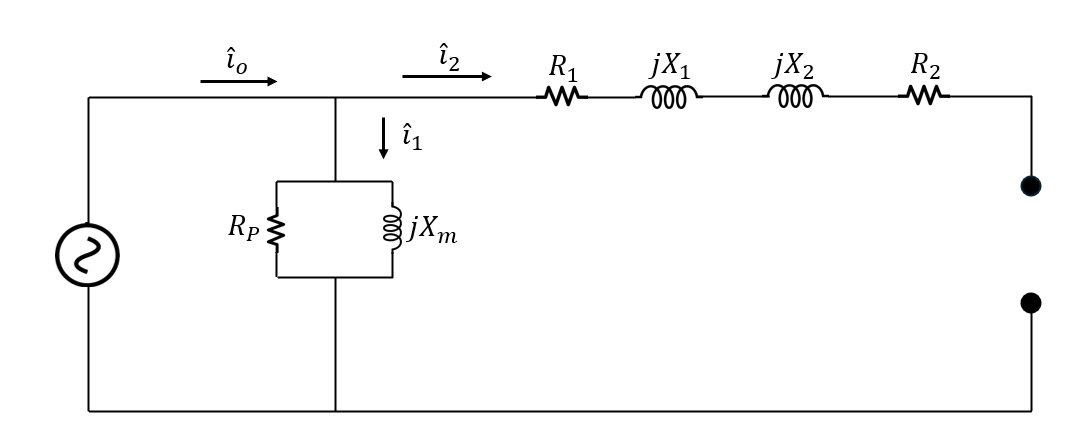
\includegraphics[width=0.6\textwidth]{Auxiliar_9_4}
        \end{center}
        \begin{center}
            \textbf{Figura 1:} Esquema del motor de induccion en su prueba al vacio
        \end{center}
        Para esta situacion se tiene el siguiente set de ecuaciones:
        \begin{align}
            R_{p} &= \frac{V_{fn}^{2}}{P_{0}}\\
            X_{n} &= \frac{V_{fn}^{2}}{Q_{0}}\\
            Q_{0} &= \sqrt{(V_{fn} \cdot I)^{2} - P_{0}^{2}}\\
        \end{align}
        Reemplazando los valores se obtiene que:
        \begin{align}
            R_{p} &= \frac{400^{2}[Vfn]}{(\sqrt{3})445[W]} = 119.8501[\Omega]\\
            Q_{0} &= \sqrt{\left(\frac{400}{\sqrt{3}} \cdot 4[A]\right)^{2} - 445[W]^{2}} = 809.5112[VAR]\\
            X_{m} &= \frac{(400/\sqrt{3})^{2}[Vfn]}{809.5115[VAR]} = 65.8834[\Omega]
        \end{align}
        Luego es posible obtener el valor de la resistencia $r_{1}$ para la prueba de corriente continua, la cual se visualiza en el siguiente esquema:
        \begin{center}
            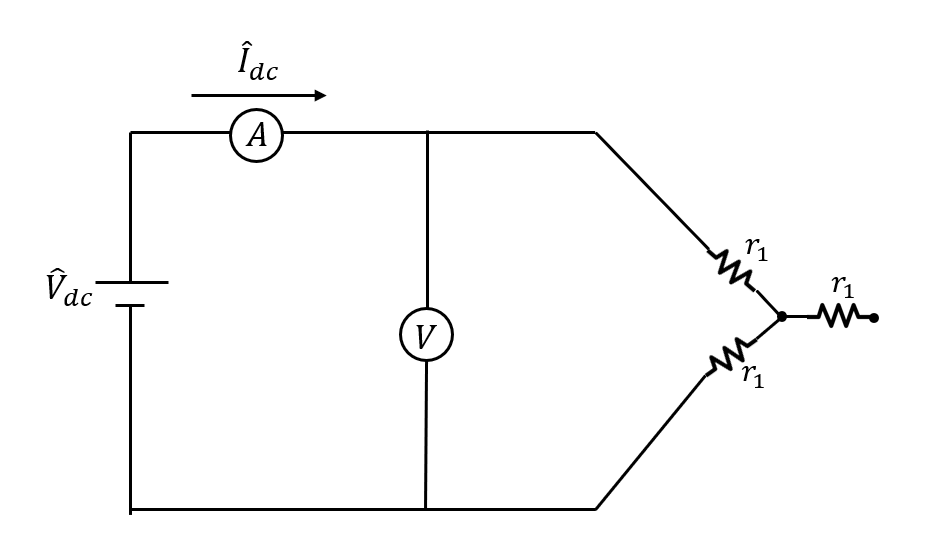
\includegraphics[width=0.5\textwidth]{Auxiliar_9_9}
        \end{center}
        \begin{center}
            \textbf{Figura 2:} Esquema del motor de induccion en su prueba de corriente continua
        \end{center}
        De esta manera se tendra que:
        \begin{align}
            2r_{1} &= \frac{V_{CD}}{I_{DC}}\\
            2r_{1} &= 1[\Omega]\\
            r_{1} &= 0.5[\Omega]
        \end{align}
        Luego, para la prueba de rotor bloqueado \textit{(la cual ocurre cuando \( w_r = 0 \), por lo que se tiene \( s = 1 \), 
        y, por tanto, la resistencia \( r_2 \) será nula, produciendo un cortocircuito)}, se tendrá el siguiente esquema:        
        \begin{center}
            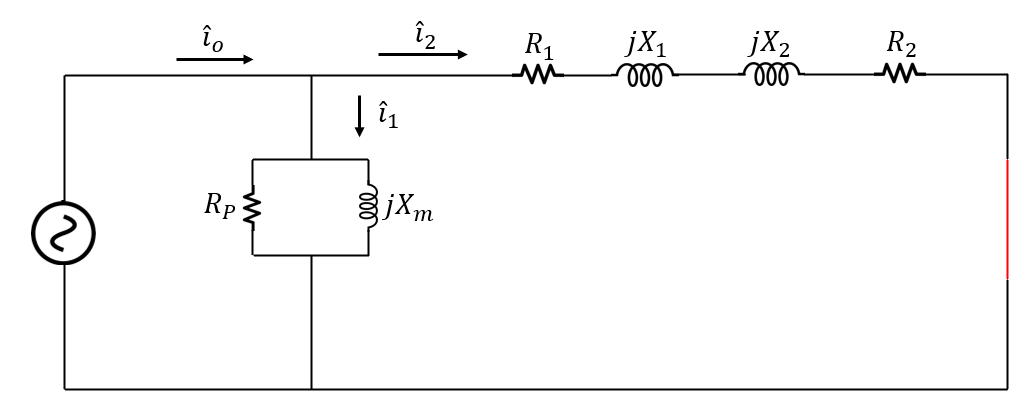
\includegraphics[width=0.6\textwidth]{Auxiliar_9_5}
        \end{center}
        \begin{center}
            \textbf{Figura 2:} Esquema del motor de induccion en su prueba de rotor bloqueado
        \end{center}
        De esta manera se deriva el sigueinte set de ecuaciones:
        \begin{align}
            r_{1} + r_{2} &= \frac{P_{cc}}{i^{2}_{cc}}\\
            X_{1} + X_{2} &= \frac{Q_{cc}}{i^{2}_{cc}}\\
            Q_{cc} &= \sqrt{(V_{cc}i_{cc})^{2} - P_{cc}^{2}}
        \end{align}
        De esta manera, reemplazando sobre los valores que se tienen se concluye que:
        \begin{align}
            r_{1} + r_{2} &= \frac{670[W]}{15[A]^{2}} = 2.977[\Omega]\\
        \end{align}
        Dado que $r_{1} = 0.5[\omega]$, luego se tiene que $r_{2} = 2.477[\omega]$.Por otro lado tenemos que:
        \begin{align}
            Q_{cc} \sqrt{ \left(\frac{400}{\sqrt{3}} \cdot 15 \right)^{2} - 670^{2}} = 640.1367[VAR]
        \end{align}
        De esta manera se tiene que:
        \begin{align}
            X_{1} + X_{2} &= \frac{640.1367[VAR]}{15[A]^{2}} = 2.844[\Omega]
        \end{align}
        Con lo que finalmente se obtienen los valores de los parametros del circuito equivalente.
        \subsection*{Resolucion 1.2}
        Se busca determine la intensidad de corriente de partida cuando el motor se conecta a una red de tensión nominal, esto quiere decir que:
        \begin{align}
            w_{r} = 0 \rightarrow s = 1 
        \end{align}
        Se tiene por tanto el siguiente esquema:
        \begin{center}
            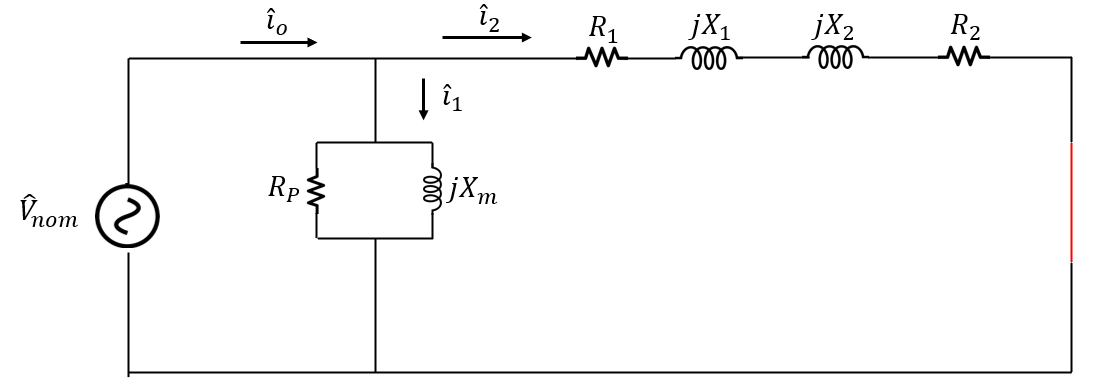
\includegraphics[width=0.6\textwidth]{Auxiliar_9_6}
        \end{center}
        \begin{center}
            \textbf{Figura 3:} Esquema del motor para la corriente de partida
        \end{center}
        De esta manera se tendra que:
        \begin{align}
            \hat{V}_{nom} = \left(\frac{400}{\sqrt{3}}\angle 0^{\circ}\right)[Vfn]= 230.94 \angle 0^{\circ}
        \end{align}
        Luego tendremos por tanto que la corriente sera:
        \begin{align}
            \hat{i}_{2} = \frac{\hat{V}_{nom}}{(r_{1} + r_{2}) + j(x_{1} + x_{2})} = 56.076 \angle -43.6944^{\circ}[A]
        \end{align}
        Con esto se tiene que:
        \begin{align}
            |i_{2}| = 56.076[A]
        \end{align}
        Con lo que se obtiene la corriente de partida.
        \subsection*{Resolucion 1.3}
        Se busca determinar la resistencia que se debe añadir en serie a cada fase del rotor para limitar la corriente de partida a \(50 \, [A]\), por lo que se tiene que:
        \begin{center}
            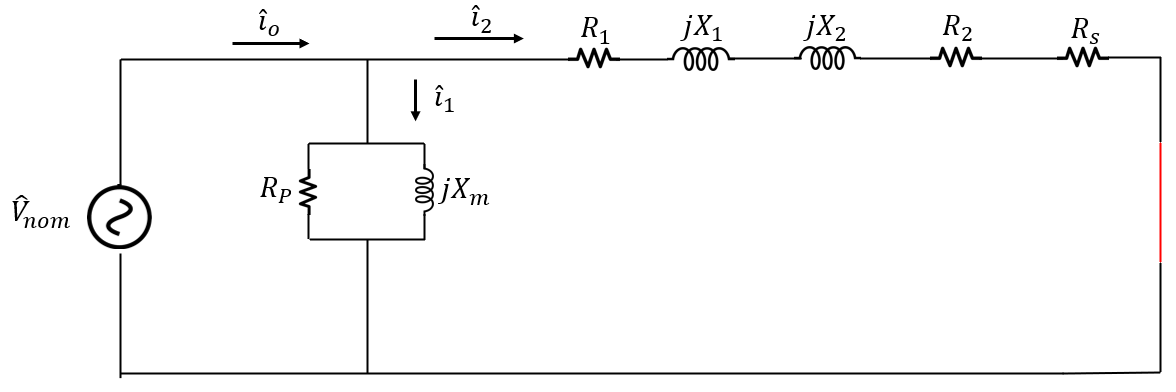
\includegraphics[width=0.6\textwidth]{Auxiliar_9_7}
        \end{center}
        \begin{center}
            \textbf{Figura 4:} Esquema del motor para la corriente de partida con una resistencia $r_{s}$ adicional
        \end{center}
        De esta manera es directo que:
        \begin{align}
            |i_{2}| = \frac{|V_{nom}|}{\sqrt{(r_{1} + r_{2} + r_{s})^{2} + (x_{1} + x_{2})^{2}}} = 50[A]
        \end{align}
        Con lo que reemplazando y despejando, se obtiene que el valor de la resistencia sera de:
        \begin{align}
            r_{s} = 0.6408[\Omega]
        \end{align}
        \subsection*{Resolucion 1.4}
        Se busca obtener la velocidad de giro, la frecuencia de las corrientes inducidas en el rotor, la corriente de la carga, la corriente de línea, la potencia consumida, las pérdidas, el factor de potencia, el rendimiento de la máquina y el torque ejercido por el eje si el deslizamiento a plena carga es del \(4 \, \%\) para lo cual consideramos que se alcanza el regimen permanente por lo que la parte transitoria es despreciable. Dado que se menciona que el deslizamiento es del 4\% se tiene que:
        \begin{align}
            s = 0.04 
        \end{align}
        Recordemos que s corresponde:
        \begin{align}
            s= \frac{w{s} - w_{r}}{w_{s}} = \frac{n_{s}- n_{r}}{n_{s}}
        \end{align}
        Con lo que considerando que:
        \begin{align}
            n_{s} = \frac{120 \cdot f}{p} = \frac{120 \cdot 50}{4} = 1500[rpm]
        \end{align}
        Con lo que podemos obtener el valor de $n_{r}$ como:
        \begin{align}
            s&= \frac{n_{s} - n_{r}}{n_{s}}\\
            0.04 &= \frac{1500 - n_{r}}{1500}\\
            n_{r} &= 1440[rpm]
        \end{align}
        Luego se tendra que en [rad/s]:
        \begin{align}
            w_{r} = \frac{2\pi n_{r}}{60} = 150.796[rad/s]
        \end{align}
        Para la frecuencia $f_{r}$ es directo que:
        \begin{align}
            f_{r} &= s \cdot f_{nom} = 0.04 \cdot 50 = 2[Hz]
        \end{align}
        Luego para la corriente de linea tenemos que recordar el esquema dado por:
        \begin{center}
            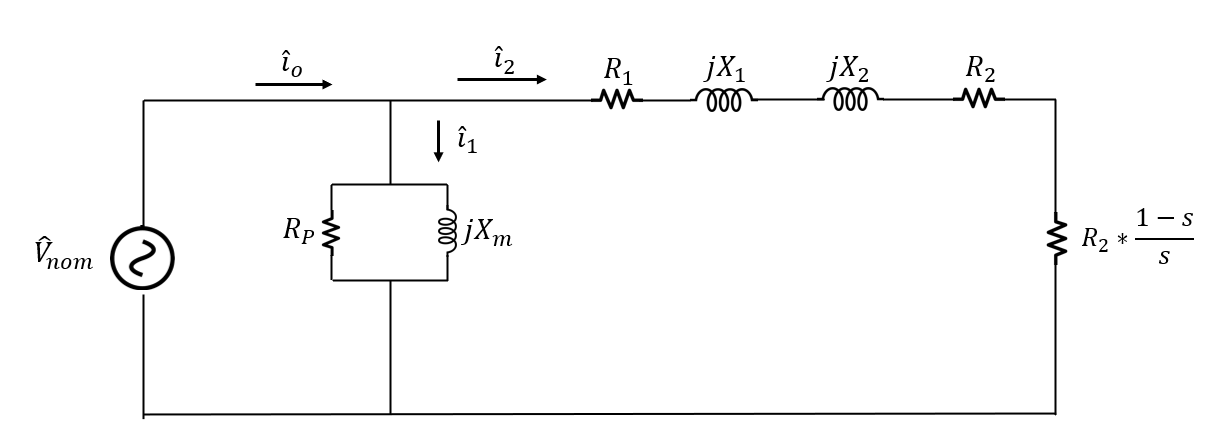
\includegraphics[width=0.6\textwidth]{Auxiliar_9_8}
        \end{center}
        \begin{center}
            \textbf{Figura 5:} Esquema del motor para la corriente de linea $i_{0}$
        \end{center}
        Tenemos que dicha corriente vendra dada por:
        \begin{align}
            \hat{i}_{0} = \frac{\hat{V}_{nom}}{Z_{eq}}
        \end{align}
        Luego tenemos que obtener el valor de la impedancia equivalente, el cual viendo el esquema se tiene:
        \begin{align}
            Z_{eq} = Z_{shunt} // Z_{serie}
        \end{align}
        donde $Z_{shunt}$ es directa de obtener en base a los valores previos, es deicr:
        \begin{align}
            Z_{shunt} &= \left( \frac{1}{R_{p}} + \frac{1}{jX_{m}}\right)^{-1}\\
            &= 57.7350 \angle 61.204^{\circ}[\Omega]
        \end{align}
        Luego se debera obtener la impedancia en serie la cual viene dada por:
        \begin{align}
            Z_{serie} = r_{1} + r_{2} + r_{2}\left(\frac{1-s}{s}\right) + j(x_{1} + x_{2}) = 62.6073 \angle 2.61^{\circ}[\Omega]
        \end{align}
        Por lo que finalmente tendremos que el valor de la impedancia equivalente sera:
        \begin{align}
            Z_{eq} = 57.7350 \angle 61.204^{\circ} // 62.6073 \angle 2.61^{\circ} = 34.4064 \angle 33.18^{\circ}[\Omega]
        \end{align}
        con lo que finalmente se obtiene que la corriente de linea sera:
        \begin{align}
            \hat{i}_{0} = \frac{230.94 \angle 0^{\circ}}{34.4064 \angle 33.18^{\circ}} = 6.71 \angle -33.18^{\circ}[A]
        \end{align}
        Luego se busca obtener la potencia consumida, ademas del factor de potencia, por lo que en base a lo ya obtenido se tiene que:
        \begin{align}
            \hat{S} = \hat{V}_{nom} \cdot \hat{i}_{0}^{*} = 1550,07 \angle 33.18^{\circ}[VA]
        \end{align}
        Con lo que es posible obtener la potencia activa y reactiva como:
        \begin{align}
            P &= Re(S) = 1550.07 \cdot cos(33.18^{\circ}) = 1297.3394[W]\\
            Q &= Im(S) = 1550.07 \cdot sen(33.18^{\circ}) = 848.5[VAR]
        \end{align}
        Con lo que es posible el identificar el factor de potencia como:
        \begin{align}
            FP = \frac{P}{|S|} = 0.838
        \end{align}
        Luego se busca obtener las potencias perdidas es decir:
        \begin{align}
            P_{perdidas} &= P_{cobre} + P_{nucleo}\\
            &= \frac{V_{nom}^{2}}{R_{p}} + |\hat{i}_{2}|^{2} \cdot(r_{1} + r_{2}) 
        \end{align}
        Por lo que se necesita obtener $\hat{i}_{2}$ como:
        \begin{align}
            \hat{i}_{2}& = \frac{\hat{V}_{nom}}{\left(r_{1} + r_{2} + r_{2}\frac{(1-s)}{s} \right)+ j(x_{1}+x_{2})}\\
            &= 3.6946 \angle -2.6087^{\circ}[A] 
        \end{align} 
        De esta manera se tiene que:
        \begin{align}
            P_{perdidas} &= \frac{(400/\sqrt{3})^{2}}{R_{p}} + 3.6946^{2} \cdot (r_{1} + r_{2}) = 485.6461[W]
        \end{align}
        Con lo que se puede obtener la potencia mecanica como:
        \begin{align}
            P_{mec} = P_{consumida} - P_{perdidas} = 1297.3394-485.6461 = 811.6933[W]
        \end{align}
        Luego con la potencia mecanica es posible el opbtener el torque mecanico como:
        \begin{align}
            T_{mec} = 3\cdot \frac{P_{mec}}{ w_{r}} = \frac{3 \cdot 811.6933[w] }{150.7964[rad/s]} = 16.1481[Nm]
        \end{align}
        Con lo que se obtieen todo lo buscado.
        \subsection*{Resolucion 1.5}
        Se busca determinar el torque maximo y el deslizamiento para esta condicion de torque maximo, estos vienen caracterizados por:
        \begin{align}
            s_{max} &= \frac{R_{2}}{\sqrt{R_{1}^{2} + (X_{1} + X_{2})^{2}}} = 0.8577\\
            T_{max} &= \frac{3p}{8\pi f} \cdot \frac{V_{1}^{2}}{R_{1}+ \sqrt{R_{1}^{2} + (X_{1} + X_{2})^{2}}} = 150.2967
        \end{align}
        El cual corresponde al caso de un motor, recordemos que:
        \begin{align}
            s>0 \quad \text{Motor} \quad s<0 \quad \text{Generador}
        \end{align}
    \end{solution}
    %---------------------------------------------------------------
    \question Obtener el diagrama en p.u. del circuito de la Figura 1.3 tomando en las líneas una potencia y tensión base de valor \(100 \, \text{MVA}\) y \(220 \, \text{kV}\) respectivamente. Las características y valores nominales para cada uno de los elementos de la red se indican en la Tabla 1.2. Además, se sabe que en el nodo 4 se consumen \(50 \, \text{Mvar}\) y \(0 \, \text{MW}\), y en el nodo 6 se consumen \(0 \, \text{Mvar}\) y \(50 \, \text{MW}\).

    \begin{figure}[H]
        \centering
        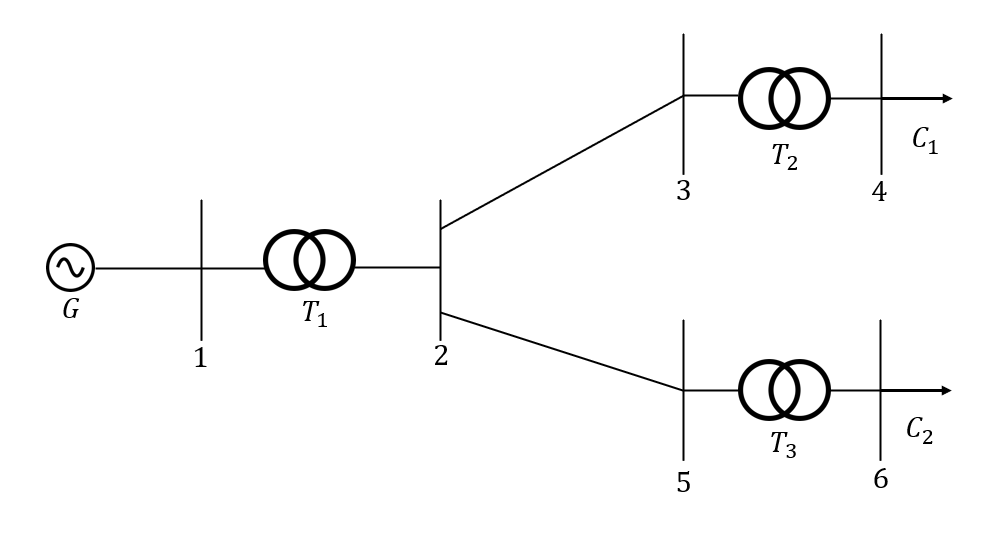
\includegraphics[width=0.6\textwidth]{Auxiliar_9_1} 
        \caption{Esquema unifilar de la red del Problema 1.2.}
    \end{figure}
    
    \begin{table}[H]
        \centering
        \caption{Datos de la red de la Figura 1.3.}
        \begin{tabular}{|c|c|c|c|}
            \hline
            \textbf{Elemento} & \(\boldsymbol{V_{\text{nom}}} \, \text{(kV)}\) & \(\boldsymbol{S_{\text{nom}}} \, \text{(MVA)}\) & \textbf{Impedancia} \\ \hline
            Generador         & \(24\)         & \(200\)   & \(X_G = 100\%\) \\ \hline
            \(T1\)            & \(25/230\)     & \(200\)   & \(X_{\text{CC}} = 10\%\) \\ \hline
            \(T2\)            & \(220/132\)    & \(150\)   & \(X_{\text{CC}} = 10\%\) \\ \hline
            \(T3\)            & \(220/66\)     & \(75\)    & \(X_{\text{CC}} = 8\%\) \\ \hline
            Línea \(2\text{-}3\) & \(-\)        & \(-\)     & \(Z = 10 + j60 \, (\Omega)\) \\ \hline
            Línea \(2\text{-}5\) & \(-\)        & \(-\)     & \(Z = 50j \, (\Omega)\) \\ \hline
        \end{tabular}
    \end{table}
    
    Si la tensión en la barra 2 es de \(231 \, \text{kV}\), determinar la potencia activa que cede el generador y las tensiones en las cargas.
    
    
    
    %---------------------------------------------------------------
    \begin{solution}
        \subsection*{Resolucion 1.1}
        Dado que se busca utilizar el diagrama en p.u. se tendra que delimitar las diferentes zonas, por lo tanto:
        \begin{center}
            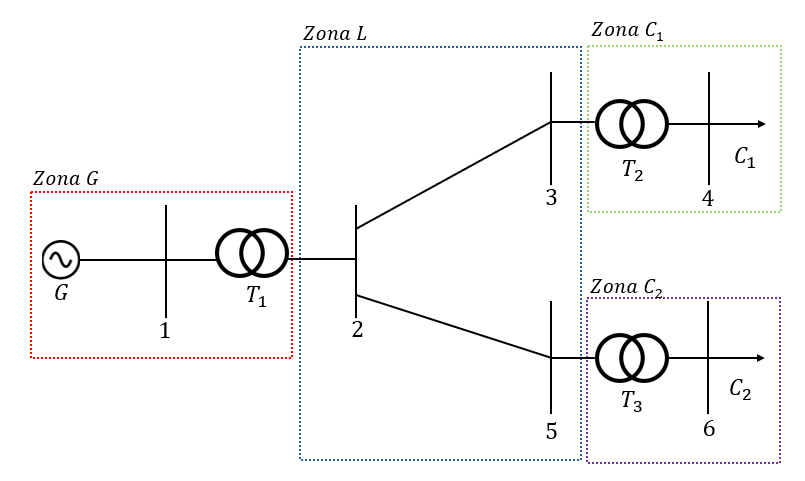
\includegraphics[width=0.6\textwidth]{Auxiliar_9_2}
        \end{center}
        Se debe tener en consideracion que la potencia base sera de 100[MVA] y la tension base de 220[kV] (\textit{La cual podemos reconocer que hace referencia a la zona L}):
        \begin{align*}
            \text{Zona L:}  & \quad V_{BL} = 220 \, \text{kV} \quad && \implies \quad Z_{BL} = \frac{220^2}{100} = 484 \, \Omega \\[10pt]
            \text{Zona G:}  & \quad V_{BG} = 220 \cdot \frac{25}{230} = 23.913 \, \text{kV} \quad && \implies \quad Z_{BG} = \frac{23.913^2}{100} = 5.718 \, \Omega \\[10pt]
            \text{Zona C1:} & \quad V_{BC1} = 220 \cdot \frac{132}{220} = 132 \, \text{kV} \quad && \implies \quad Z_{BC1} = \frac{132^2}{100} = 174.24 \, \Omega \\[10pt]
            \text{Zona C2:} & \quad V_{BC2} = 220 \cdot \frac{66}{220} = 66 \, \text{kV} \quad && \implies \quad Z_{BC2} = \frac{66^2}{100} = 43.56 \, \Omega
            \end{align*}
        Es importante mencionar que dado que nos ubicamos en la zona L, se debe tener el cuidado con la relaciones de los transformados, dado que dependera si pasamos de una zona de baja tension a una de alta tension o viceversa. Por otro lado es posible obtener las impedancias de lineas como:
        \begin{align}
            Z_{23} &= \frac{10+60j}{Z_{BL}} = \frac{10+60j}{484} = 0.021 + 0.1241j \, \Omega \\
            Z_{25} &= \frac{50j}{Z_{BL}} = \frac{50j}{484} = 0.1033j \, \Omega
        \end{align}
        Luego es posible el obtener la impedancia del generador a por unidad p.u. considerando que este tiene un 100\% de reactancia equivalente a 1:
        \begin{align}
            X_{G} &= 1\cdot \frac{\frac{24^{2}}{200}}{Z_{BG}}\\
             &= \frac{\frac{24^{2}}{200}}{5.718} = 0.504 
        \end{align}
        De la misma manera se obtiene la impedancia de los transformadores en por unidad como:
        \begin{align}
            X_{T1} &= 0.1 \cdot \frac{\frac{25^{2}}{200}}{Z_{BG}} = 0.055\\
            X_{T2} &= 0.1 \cdot \frac{\frac{220^{2}}{150}}{Z_{BL}} = 0.067\\
            X_{T3} &= 0.08 \cdot \frac{\frac{66^{2}}{75}}{Z_{BC2}} = 0.107
        \end{align}
        Luego utilizando la potencia base, es posible obtener las potencias en las cargas, teniendo el cuidado en las unidades de medida, para saber si se habla de potencia activa o reactiva, de tal manera:
        \begin{align}
            S_{C1} &= \frac{50j}{S_{B}} = 0.5j\\
            S_{C2} &= \frac{50}{S_{B}} = 0.5
        \end{align}
        De esta manera se tendra el sigueinte esquema:
        \begin{center}
            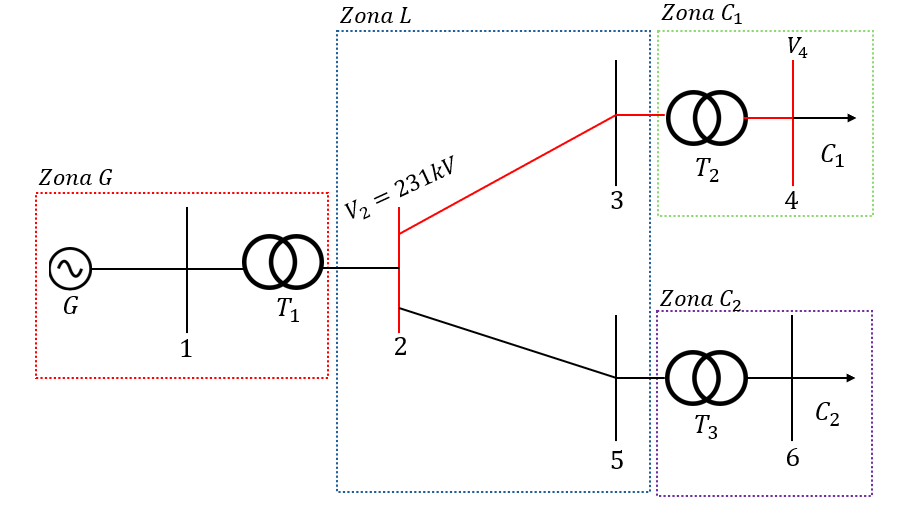
\includegraphics[width=0.6\textwidth]{Auxiliar_9_3}
        \end{center}
        Luego se debe normalizar el voltaje de la barra 2, por lo que se tiene que:
        \begin{align}
            \hat{V_{2}} &= \frac{231}{220} = 1.05
        \end{align}
        Luego podemos utilizar ley de kirchoff para obtener la corriente en la barra 2, donde debemos considerar que la corriente que cirula por esa linea dara cuenta de la impedancia de linea 2-3 y la impedancia del transformador 2, por tanto:
        \begin{align}
            \hat{V_{2}} - \hat{V_{4}} &= \hat{I}_{C1} \cdot (Z_{23} + X_{T2})\\
            \hat{V}_{2} &= \hat{V}_{4} + \hat{I}_{C1} \cdot (Z_{23} + X_{T2})\\
        \end{align}
        Por otro lado tenemos que la corriente se puede obtener como:
        \begin{align}
            \hat{I}_{C1} = \left( \frac{0.5j}{\hat{V_{4}}}\right)^{*}
        \end{align}
        Por lo que reemplazando se obtiene:
        \begin{align}
            \hat{V}_{2} &= \hat{V}_{4} + \hat{I}_{C1} \cdot (Z_{23} + X_{T2})\\
            \hat{V}_{2} &= \hat{V}_{4} + (Z_{23} + X_{T2})\cdot \frac{-0.5j}{\hat{V}^{*}_{4}}
        \end{align}
        Luego es posible reemplazar los valores de las impedancias tal que 
        \begin{align}
            \hat{V}_{2} &= \hat{V}_{4} + (0.021+0.1241j + 0.067j)\cdot \frac{-0.5j}{\hat{V}^{*}_{4}}\\
            &=\hat{V}_{4} + (0.021+0.191j)\cdot \frac{-0.5j}{\hat{V}^{*}_{4}}\\
            &= \frac{0.0955-0.0105j}{\hat{V}^{*}_{4}} + \hat{V}_{4}
        \end{align}
        Luego se utilizara como referencia el la barra 4, es decir que los desfases seran vistos con respecto a esta, de esta manera se obtiene que:
        \begin{align}
            U_{4} &= \hat{V}_{4}\angle 0\\
            \hat{V}_{2} &= 1.05 \angle \theta
        \end{align}
        Esto permite que el conjugado sea no sea relevante dado que la fase sera 0 y por tanto es posible obtener que:
        \begin{align}
            \hat{V}_{2} &= \left(\frac{0.0955}{V_{4}}\right) - j\left(\frac{0.0104}{V_{4}}\right) + V_{4}
        \end{align}        
        Luego separando la componente real e imaginaria se tiene respectivamente:
        \begin{align}
            1.05 \cdot cos(\theta) &= \frac{0.0955}{U_{4}} + U_{4}\\
            1.05 \cdot sin(\theta) &= -\frac{0.0104}{U_{4}}
        \end{align}
        Luego resolviendo las ecuaciones se logra obtener que:
        \begin{align}
            U_{4} &= 0.95 \angle 0\\
            \hat{V}_{2} &= 1.05 \angle (-0.594)
        \end{align}
        Realizando el calculo analogo es posible obtener el voltaje en la barra 6 similar a lo anterior, considerando que:
        \begin{align}
            S_{C2} &= \hat{V}_{6} \cdot I_{C2}^{*}  
        \end{align}
        Por lo que se debe obtener la corriente la cual vendra dada por:
        \begin{align}
            i_{C2} = \frac{\hat{V}_{2} - \hat{V}_{6}}{Z_{25 + X_{T3}}}
        \end{align}
        Es decir:
        \begin{align}
            S_{C2} &= \hat{V}_{6} \cdot I_{C2}^{*}\\
                   &= \hat{V_{6}} \cdot \frac{\hat{V}_{2} - \hat{V}_{6}}{Z_{25} + X_{T3}}\\ 
        \end{align}
        Luego trabajando las expresiones en su parte real e imaginaria respectivamente se logra obtener que:
        \begin{align}
            P_{6} &= 0.5 = \frac{1.05 \hat{V}_{6}}{X_{25} + X_{T3}} \cdot sen(\theta_{2} - \theta_{6})\\
            Q_{6} & = 0  =\frac{1.05 \hat{V}_{6}}{X_{25} + X_{T3}} \cdot cos(\theta_{2} - \theta_{6}) - \frac{\hat{V}_{6}^{2}}{X_{25} + X_{T3}} 
        \end{align}
        con lo que es posible obtener que:
        \begin{align}
            \hat{V}_{6} &= 1.048 \angle -3.55
        \end{align}
        Con lo que finalmente dado que se busca obtener la potencia activa que cede el generador, se tiene que sera la potencia consumida por la carga C2 (\textit{Dado que en C1 solo tenemos potencia reactiva}), mas las perdidas en el tramo de linea 2-3 dado que es la unica que presenta resistencia, por lo que:
        \begin{align}
            P_{G} &= P_{C2} + R_{23} \cdot I_{23}^{2}\\
                  &= 0.5 + 0.021 \cdot \frac{0.5^{2}}{V_{4}^{2}} = 0.50573[p.u]\\
                  &= 50.573[MW]  
        \end{align}
        Con lo que finalmente se obtiene la potencia activa que cede el generador.
    
       
    \end{solution}
    %%%%%%%%%%%%%%%%%%%%%%%%%%%
%----------------------------
\end{questions}
\newpage
%%%%%%%%%%%%%%%%%%%%%%%%%%%


\end{document}